\section{Cook-Levin}%
\label{sec:cooklevin}

\begin{frame}
	\frametitle{Pensum}
	\begin{itemize}
		\item Sipser 7.4: \textbf{Bevis at CNF-SAT er NP-Komplet}
		\item Weekly Note 9
		\item Video 18 (Bonus \href{https://www.youtube.com/watch?v=6Az1gtDRaAU}{video})
	\end{itemize}
\end{frame}

\begin{frame}[allowframebreaks]
	\frametitle{Cook-Levin}
	\begin{definition}
		$B$ er $NP$-komplet hvis:
		\begin{enumerate}
			\item $B \in NP$
			\item $\forall A \in NP, A \le_{P} B$
		\end{enumerate}
	\end{definition}
	\begin{itemize}
		\item Man antager generelt at $P \ne NP$, så derfor hvis vi beviser NP-Komplethed for et problem, beviser vi at der nok ikke er en polynomiel algoritme der kan løse problemet.
	\end{itemize}

	\begin{center}
		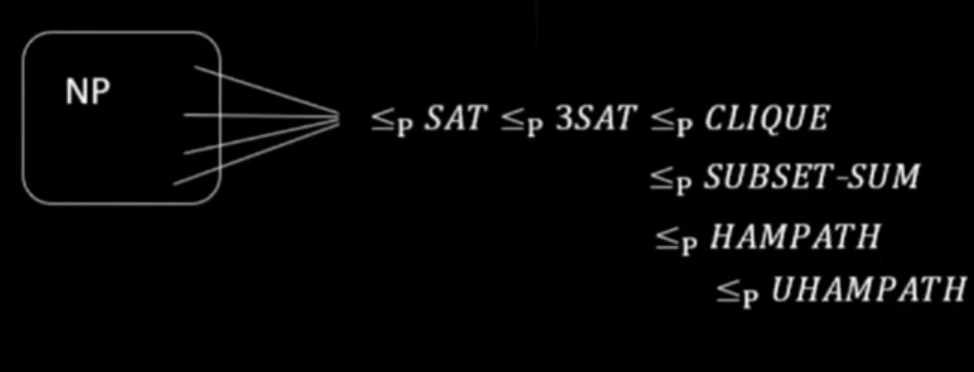
\includegraphics[scale=0.4]{figur/video16a.png}
	\end{center}

	\begin{itemize}
		\item Reminder: \(\sum_{1 \le i \le n}i = 1 + 2+ \cdots + n\)
		\item På samme måde hvis $x = x_{1} \cdots x_{n}$ og $y = y_{1} \cdots y_{n}$, hvornår gælder følgende så?
		      \begin{equation}
			      \left( \bigwedge_{1 \le i \le n} x_{i} = y_{1} \right) = True
		      \end{equation}
		\item Svar: Når $x = y$!
		\item Altså bliver den til udtrykket $(x_{1} = y_1) \land (x_{2} = y_2) \land \cdots \land (x_{k} = y_{k})$
		\item Til gengæld, hvis det var følgende udtryk i stedet:
		      \begin{equation}
			      \left( \bigvee_{1 \le i \le n} x_{i} = y_{1} \right) = True
		      \end{equation}
		\item Ville svaret være når $x_{i} = y_{i}$ for en eller anden $i$.
		\item Nu er vi ved at være klar!
	\end{itemize}

	\begin{theorem}
		$SAT$ er $NP$-komplet.
	\end{theorem}
	\begin{itemize}
		\item Jeg bruger (sandsynligvis) udelukkende Sipsers \href{https://youtu.be/6Az1gtDRaAU}{video forelæsning}. Det vil sige at hverken Jørgens noter, eller bogen er brugt til dette.
		\item Beviset er faktisk ikke så svært! Det er bare meget langt.
		\item For at bevise sætningen, skal vi bevise to ting:
		      \begin{enumerate}
			      \item $SAT \in NP$ (allerede gjort, hvis ikke bliver det gjort i spørgsmål 5 når jeg er færdig med den.)
			      \item $\forall A \in NP : A \le_{P} SAT$.
		      \end{enumerate}

		\item Givet en $A \in NP$ som afgøres af en NDTM i tid $n^{k}$ altså polynomiel.
		\item Vores mål er at give en reduktion i polynomiel tid $f$ som mapper $A$ til $SAT$.
		\item Måden denne fungerer på er ved at mappe strenge som \textit{måske} er i $A$ til sandhedsformler som \textit{måske} er satisfiable.
		\item $f : \Sigma^{*} \longrightarrow \text{ formler }$
		\item $f(w) = \langle \phi_{M,w} \rangle$
		\item $w \in A \iff \phi_{M,w}$ er satisfiable.
		\item Så altså er vores mål at lave en reduktion der reducerer så en streng er i $A$ \textbf{hvis og kun hvis} den resulterende formel er satisfiable.
		\item Vores idé er at lade $\phi_{M,w}$ \textit{simulere} $M$ på $w$, så vi designer \(\phi_{M,w}\) til at ``sige'' at $M$ accepterer $w$.
		\item Så man kan se \(\phi_{M,w}\) som et statement: ``$M$ accepterer $w$'', og resultatet er så enten \textit{sandt} eller \textit{falsk}.
	\end{itemize}

	\begin{definition}
		En (accepterende) tableau for en NDTM $M$ på $w$ er en tabel af størrelse $n^{k} \times n^{k}$, som repræsenterer en \textit{komputeringshistorie} for $M$ på $w$ på en accepterende gren af den nondeterministiske komputering.
	\end{definition}
	\begin{center}
		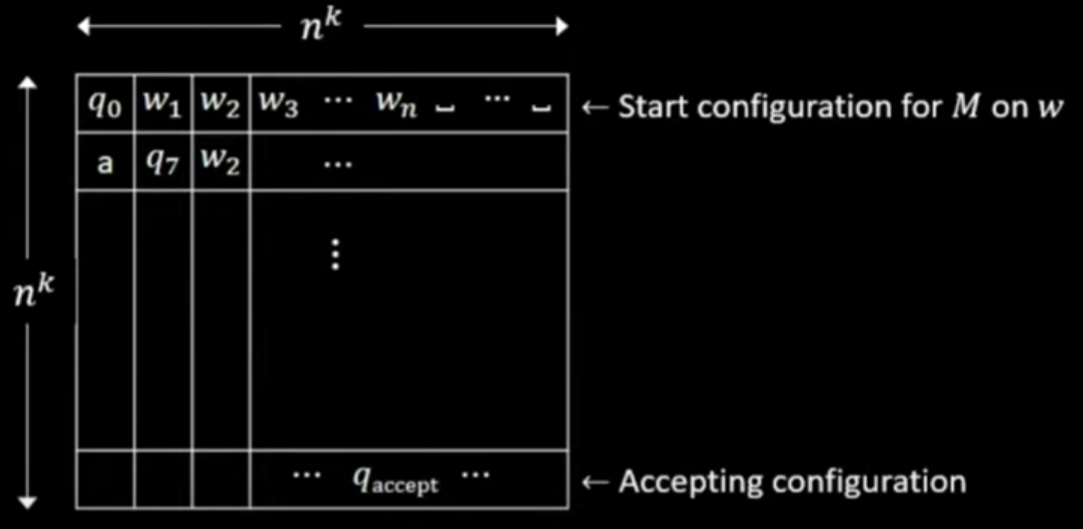
\includegraphics[scale=0.45]{figur/video16b.png}
	\end{center}

	\begin{itemize}
		\item Det betyder altså at denne tableau er en ``historie'' for hvordan $M$ kører på $w$ og accepterer $w$.
		\item Hver række er altså en konfiguration af maskinen.
		\item Række 2 viser altså en mulig næste konfiguration hvor den næste tilstand er $q_{7}$, den er rykket én til højre, og har ændret $w_{1}$ til $a$.
		\item Størrelsen på tabellen kommer fra at maskinen har køretid $n^{k}$, så dermed kan den højest køre i $n^{k}$ skridt, og højest lave $n^{k}$ ændringer på båndet.
		\item Det er \textbf{vigtigt} at huske at en tableau kun er én accepterende gren, ikke alle grene!
		\item Vores mål er nu at konstruere \(\phi_{M,w}\) til at ``sige'' at $M$ accepterer $w$, og altså dermed sige at der eksisterer en tableau $M$ på $w$.
		\item Husk at vi her antager at en tableau er \textit{accepterende}.
		\item Måden vi kommer til at konstruere denne formel på er i skridt, som følger: \(\phi_{M,w} = \phi_{cell} \land \phi_{start} \land \phi_{move} \land \phi_{accept}\)
		\item Så altså siger \(\phi_{M,w}\) at:
		      \begin{enumerate}
			      \item \(\phi_{cell}\): Cellerne er korrekte
			      \item \(\phi_{start}\): Den starter korrekt
			      \item \(\phi_{move}\): Den bevæger sig korrekt
			      \item \(\phi_{accept}\): Den ender korrekt
		      \end{enumerate}
		\item Bare rolig, det er ikke meningen at noget af dette skal give mening endnu.
	\end{itemize}
\end{frame}

\begin{frame}[allowframebreaks]
	\frametitle{Konstruktion af \(\phi\): \(\phi_{cell}\)}
	\begin{center}
		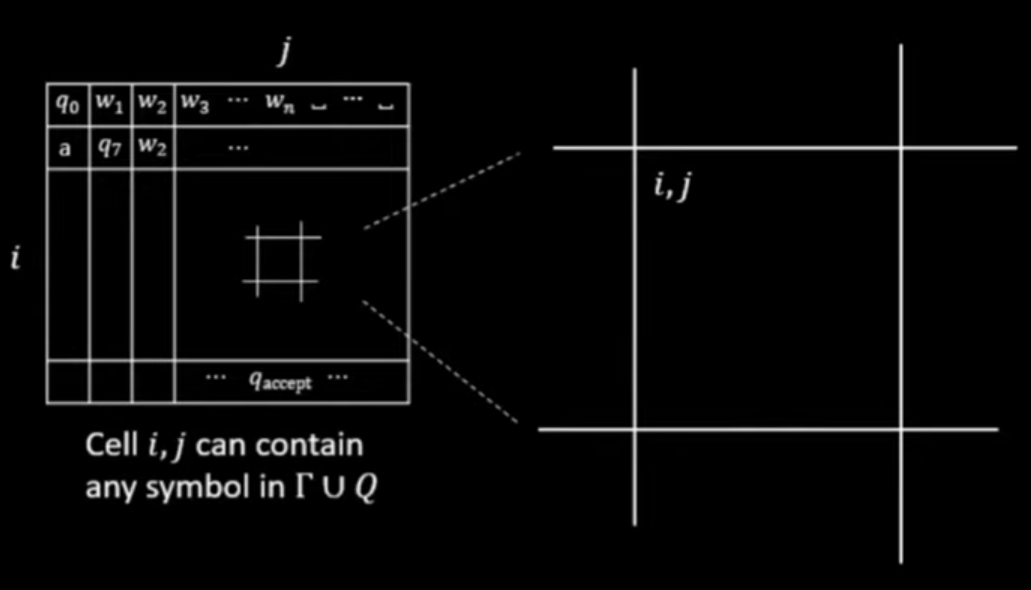
\includegraphics[scale=0.3]{figur/video16c.png}
	\end{center}
	\begin{itemize}
		\item Variablerne i \(\phi_{M,w}\) er $x_{i,j,\sigma}$ for $1 \le i,j \le n^{k}$ og $\sigma \in \Gamma \cup Q$
		\item Det vil altså sige at der er en variabel for én af hvert symbol $\sigma \in \Gamma \cup Q$.
	  \item Dette er fordi, en konfiguration er en blanding af båndsymboler og tilstande.
		\item Hvis $x_{i,j,\sigma} = \text{\texttt{True}}$, betyder det at cellen $i,j$ indeholder symbolet \(\sigma\).
	  \item Så, hvis $i,j$ indholder $a$, så vil $x_{i,j,a} = True$, men $x_{i,j,\sigma}$ hvor $\sigma = (\Gamma \cup Q) \setminus \{a\}$ ville være falsk.
	  \item Det introducerer altså en regel: Hver celle må \textbf{højest} have én sand værdi.
	  \item På samme tid, trods der kun må være én sand værdi, skal det også \textbf{mindst} være en sand værdi!
	  \item Måden vi sikrer at der mindst er en sand værdi:
			\begin{equation}
x_{i,j,\sigma_{1}} \lor x_{i,j,\sigma_{2}} \lor \cdots \lor x_{i,j,\sigma_{t}}
			\end{equation}
	  \item Som vi kan skrive således:
			\begin{equation}
\bigvee_{\sigma \in \Gamma \cup Q} x_{i,j,\sigma}
			\end{equation}
	  \item Vi vil også sikre at er \textit{højest} er én sand variabel:
			\begin{equation}
\bigwedge_{\sigma, \tau \in \Gamma \cup Q, \sigma \ne \tau} (\overline{x_{i,j,\s} \land x_{i,j,\tau}})
			\end{equation}

	  \item Altså for alle to forskellige symboler, \(\sigma\) og \(\tau\) må de \textbf{ikke} være sande.
	  \item Måden vi får en formel der kigger for begge disse, er bare ved at putte dem sammen via en $\lor$ operation, således:
			\begin{equation}
\left(  \bigvee_{\sigma \in \Gamma \cup Q} x_{i,j,\sigma} \right) \land \left(    \bigwedge_{\sigma, \tau \in \Gamma \cup Q, \sigma \ne \tau} (\overline{x_{i,j,\s} \land x_{i,j,\tau}}) \right)
			\end{equation}
	  \item Vi vil gerne have at denne operation skal laves over \textit{alle} mulige celler:
			\begin{equation}
\bigwedge_{1 \le i,j \le n^{k}} \left( ... \right)
			\end{equation}
	  \item Så vi ender altså med en formel for \(\phi_{cell}\) som følger:
			\begin{equation}
			  \bigwedge_{1 \le i,j \le n^{k}} \left(
\left(  \bigvee_{\sigma \in \Gamma \cup Q} x_{i,j,\sigma} \right) \land \left(    \bigwedge_{\sigma, \tau \in \Gamma \cup Q, \sigma \ne \tau} (\overline{x_{i,j,\s} \land x_{i,j,\tau}}) \right)
			  \right)
			\end{equation}
	\end{itemize}
\end{frame}

\begin{frame}
  \frametitle{Konstruktion af \(\phi\): \(\phi_{start}\), \(\phi_{accept}\)}
\begin{itemize}
  \item I sin essens:
		\begin{itemize}
		  \item \(\phi_{start}\) siger at startkonfigurationen skal være $q_{0}w_{1}\ldots w_{n} \sqcup \ldots \sqcup$
		  \item \(\phi_{accept}\) siger at den sidste konfiguration skal være en valid acceptkonfiguration $ \cdots q_{accept} \cdots$.
		\end{itemize}

  \item Måden vi laver \(\phi_{start}\) på er simpelt:
		\begin{equation}
\phi_{start} = x_{1,1,q_{0}} \wedge x_{1,2,w_{1}} \wedge \cdots \wedge x_{1,n+1,w_{n}} \wedge \cdots \wedge x_{1,n^{k}, \sqcup}
		\end{equation}
  \item \(\phi_{accept}\) er på samme måde meget simpelt:
		\begin{equation}
\bigvee_{1 \le j \le n^{k}} x_{n^{k}},j,q_{accept}
		\end{equation}

  \item Altså skal bare én af disse være $q_{accept}$.
\end{itemize}
\end{frame}

\begin{frame}[allowframebreaks]
  \frametitle{Konstruktion af \(\phi\): \(\phi_{move}\)}
\begin{itemize}
  \item \(\phi_{move}\) skal sikre sig at hver ændring af konfigurationen fra et skridt til det næste, er lovligt.
  \item Måden vi gør dette på er ved at bruge ``neighbourhoods'' eller ``nabolag'', som er $2\times3$ celler i tableauen.
		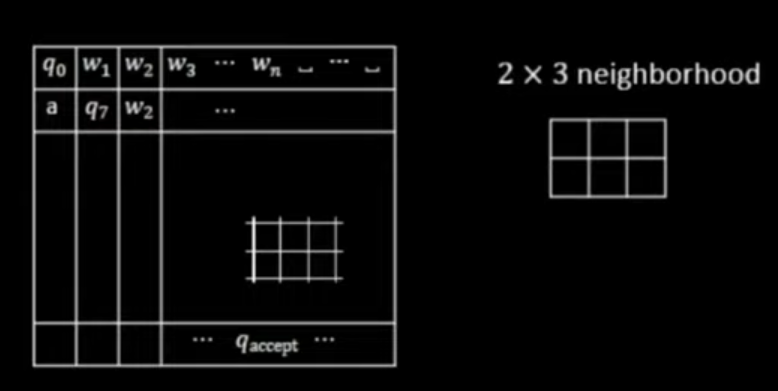
\includegraphics[scale=0.4]{figur/video16d.png}
  \item Move er i sin essens relativt simpelt: Hvis alle 3 celler er lovlige, og vi går igennem alle mulige neighbourhoods, så er hele bevægelsen lovlig.
  \item Følgende er eksempler på lovlige og ulovlige nabolag:
		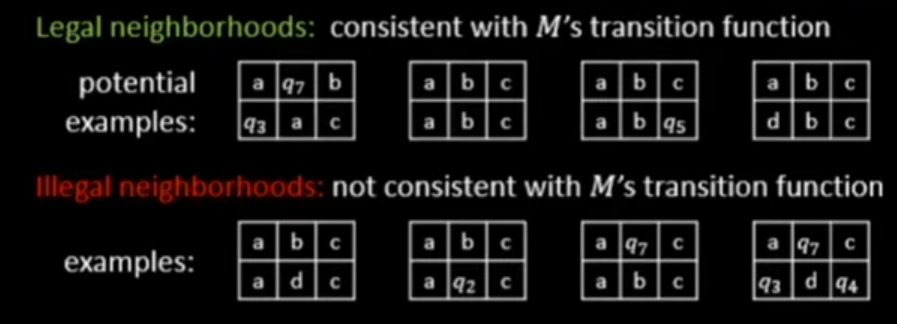
\includegraphics[scale=0.4]{figur/video16e.png}

  \item \textbf{Spørgsmål}: Hvorfor er den sidste ulovlig, når det er en NDTM?
  \item Det sidste eksempel er også grunden til at et $2 \times 2$ nabolag ikke er nok.
  \item Vi laver så dette til en boolsk formel, givet et nabolag $((r,s,t),(v,y,z))$:
		\begin{equation}
\bigvee_{Lovlig}  (x_{i,j-1,r} \wedge x_{i,j,s} \wedge x_{i,j+1,t} \wedge x_{i+1,j-1,v} \wedge x_{i+1,j,y} \wedge x_{i+1,j+1,z})
		\end{equation}
  \item Vi vil så gerne gøre dette for alle mulige $i,j$ så vi ved at hele tableauen's overføringsfunktion er korrekt:
		\begin{align*}
		  \phi_{move} = \bigwedge_{1 < i,j < n^{k}}& \Big( \bigvee_{Lovlig} (x_{i,j-1,r} \wedge x_{i,j,s} \wedge  \\
		  &x_{i,j+1,t} \wedge x_{i+1, j-1, v} \wedge x_{i+1,j,y} \wedge x_{i+1,j+1,z}) \Big)
		\end{align*}
  \item Bemærk her at $\bigvee_{Lovlig}$ betyder at den tager alle lovlige nabolag, og ser om det er en af dem.
  \item Der er kun en endelig del af disse, $|\Gamma \cup Q|^{6}$.
  \item Til sidst: Vi kigger på noterne vi må bruge til eksamen, og ``oversætter''.
\end{itemize}
\end{frame}

%%% Local Variables:
%%% mode: latex
%%% TeX-engine: xetex
%%% TeX-command-extra-options: "-shell-escape"
%%% TeX-master: "main"
%%% End:
